\documentclass[10pt,a4paper]{report}
\usepackage[utf8]{inputenc}
\usepackage[russian]{babel}
\usepackage{amsmath}
\usepackage{amsfonts}
\usepackage{amssymb}
\usepackage{graphicx}
\renewcommand{\thesection}{\arabic{section}}
\setcounter{totalnumber}{10}
\setcounter{topnumber}{10}
\setcounter{bottomnumber}{10}
\renewcommand{\topfraction}{1}
\renewcommand{\textfraction}{0}
\author{Евсеев Дмитрий}
\title{Лабораторная работа №3.\\
	Программа для шифрования и подписи GPG, пакет Gpg4win}
\begin{document}
	\maketitle
	\tableofcontents
	\pagebreak
	
	\section{Цель работы}
	Научиться создавать сертификаты, шифровать файлы и ставить ЭЦП.
	
	\section{Описание работы}
	Электронная подпись (ЭП) – это особый реквизит документа, который позволяет установить отсутствие искажения информации в электронном документе с момента формирования ЭП и подтвердить принадлежность ЭП владельцу. Значение реквизита получается в результате криптографического преобразования информации.
	
	\section{Ход работы}
	Работа на данном этапе производится во frontend для gpg kleopatra. Kleopatra — инструмент для управления сертификатами X.509 и ключами pgp.
	
	\subsection{Создание ключевой пары gpg}
	Во вкладке \textit{"File"} выбираем \textit{"New certificate"}. В открывшемся окне вводим информацию: имя ключа, адрес почты, комментарии (рисунок \ref{Img:1}).
	
		\begin{figure}[h]	
			\center{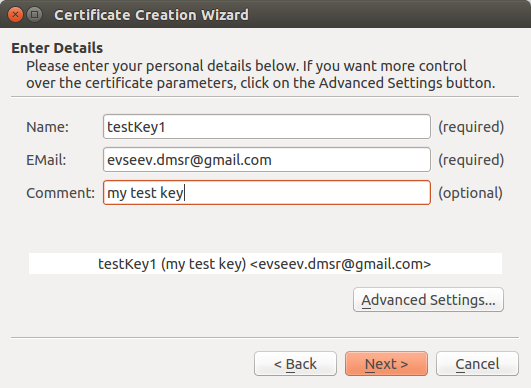
\includegraphics[width=0.8\linewidth]{Img/1}}
			\caption{Окно для ввода персональных данных.}
			\label{Img:1}
		\end{figure}
	
	Далее открывается окно подтверждения, в котором можно еще раз проверить информацию (рисунок \ref{Img:2})
	
		\begin{figure}[h]	
			\center{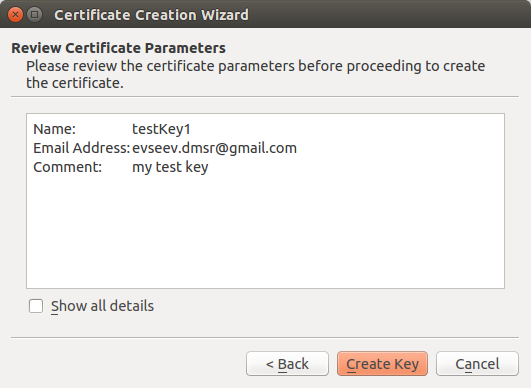
\includegraphics[width=0.8\linewidth]{Img/2}}
			\caption{Окно подтверждения.}
			\label{Img:2}
		\end{figure}
	
	Далее система просит ввести фразу-пароль. Появляется предупреждение о том, что программе нужно генерировать большое множество псевдослучайных величин и для этого не плохо было бы вести активную работу (перемещать мышь, печатать и т. д.), увеличивая тем самым энтропию (рисунок \ref{Img:3})
	
		\begin{figure}[h]	\center{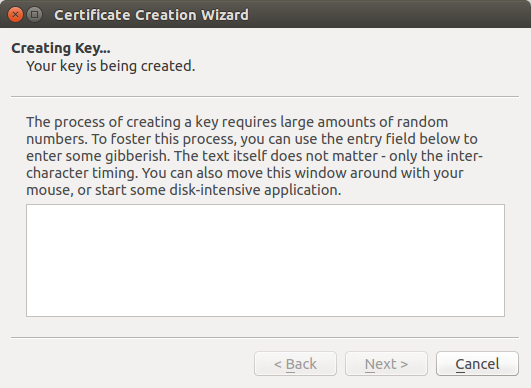
\includegraphics[width=0.8\linewidth]{Img/3}}
			\caption{Информационное окно.}
			\label{Img:3}
		\end{figure}
		
	Теперь можно увидеть новый сертификат в списке всех сертификатов (рисунок \ref{Img:4})
	
		\begin{figure}[h]
			\center{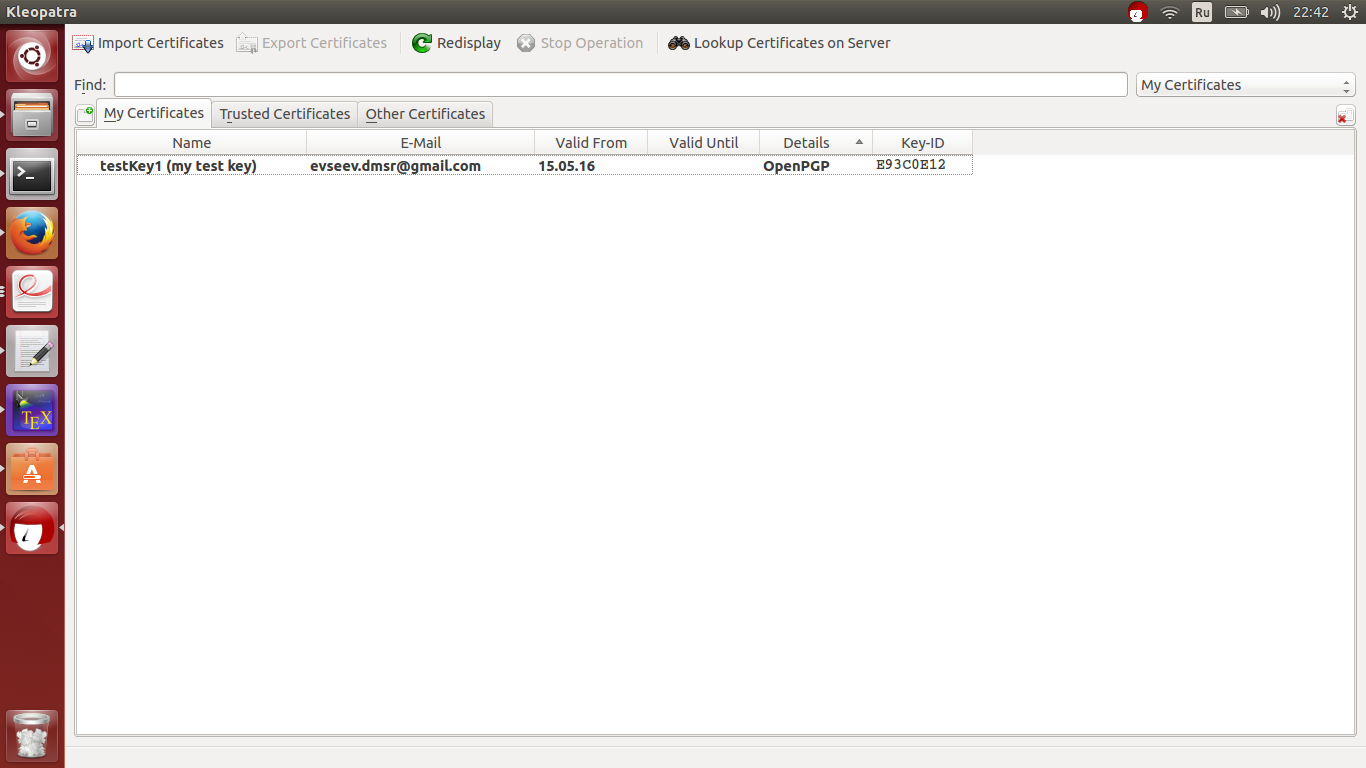
\includegraphics[width=0.8\linewidth]{Img/4}}
			\caption{Список сертификатов.}
			\label{Img:4}
		\end{figure}
		\pagebreak
		
	\subsection{Экспорт сертификата}
	Для экспорта сертификата во вкладке \textit{"File"} выбираем \textit{"Export Certificate"}. После чего введем имя файла \textit{testKey.asc} (рисунок \ref{Img:5}).
	
		\begin{figure}[h]
			\center{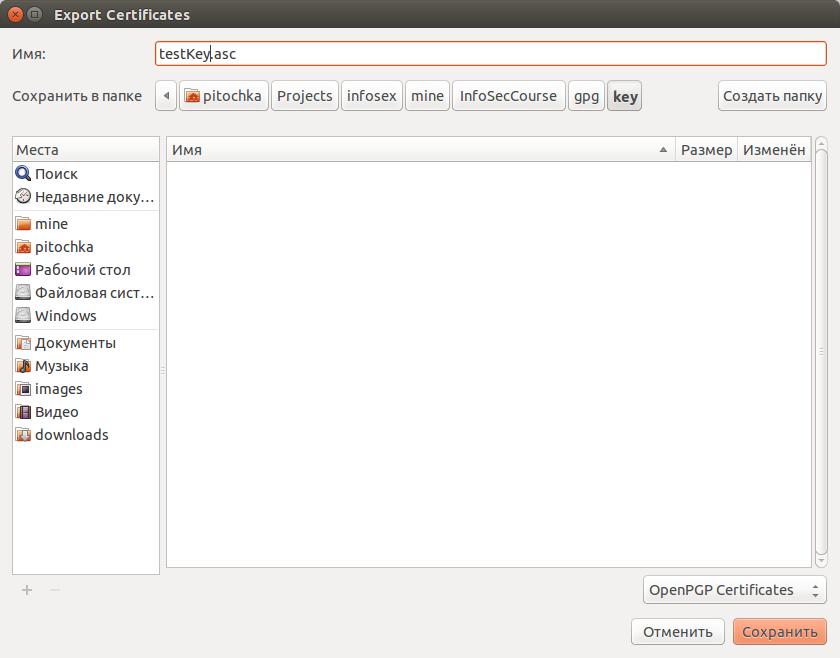
\includegraphics[width=0.7\linewidth]{Img/5}}
			\caption{Экспорт сертификата.}
			\label{Img:5}
		\end{figure}
	
	\subsection{Постановка ЦП на файл}
	Для того, что бы поставить ЦП, во вкладке  \textit{"File"} выбираем \textit{"Sign/Encrypt Files"} и выберем файл, на который необходимо поставить ЭЦП.В нашем случае это \textit{readme.txt} (рисунок \ref{Img:6}).
	
		\begin{figure}[h]
			\center{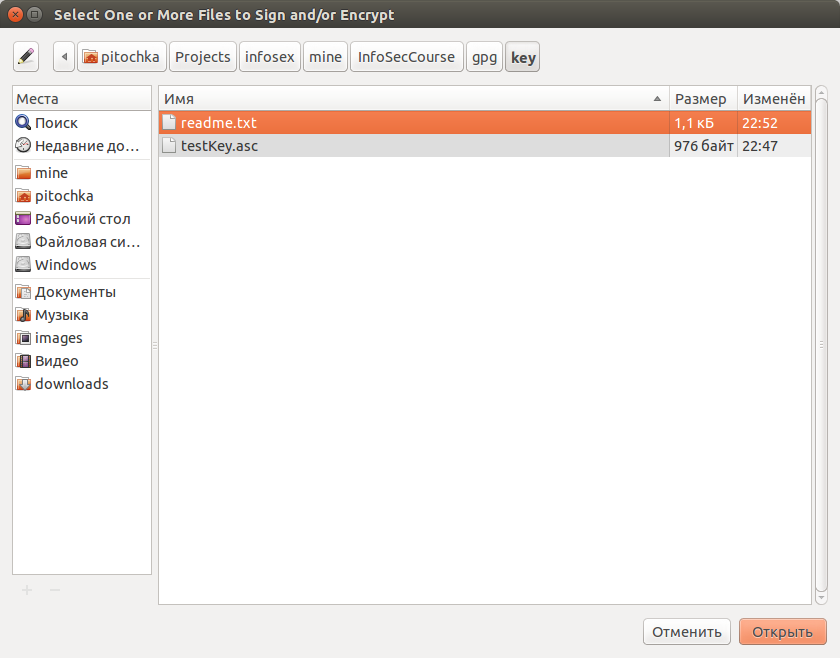
\includegraphics[width=0.7\linewidth]{Img/6}}
			\caption{Установка ЦП.}
			\label{Img:6}
		\end{figure}
	
	После выберем одно из трех предложенных действий.
	\begin{itemize}
		\item Sign and Encrypt
		\item Encrypt
		\item Sign
	\end{itemize} 
	В нашем случае \textit{Sign} - создание цифровой подписи (рисунок \ref{Img:7})
			
		\begin{figure}[h]
			\center{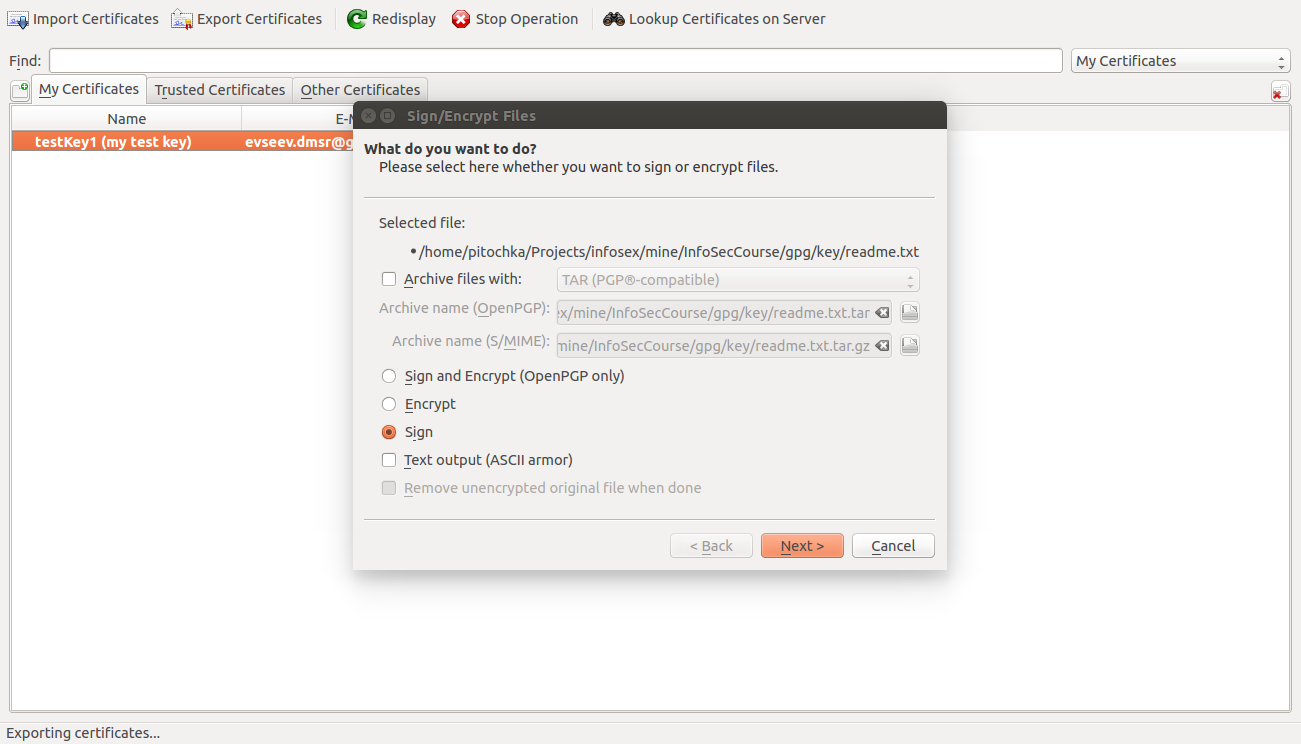
\includegraphics[width=0.7\linewidth]{Img/7}}
			\caption{Выбор стандарта и сертификата.}
			\label{Img:7}
		\end{figure}
			
	В открывшемся окне выбираем стандарт и один из имеющихся сертификатов(рисунок \ref{Img:8}).
	
		\begin{figure}[h]
			\center{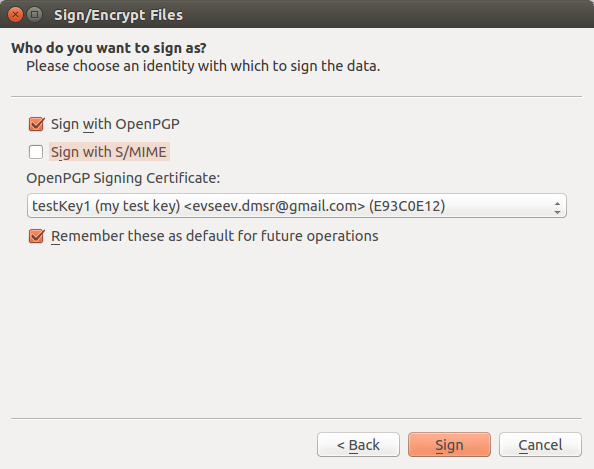
\includegraphics[width=0.8\linewidth]{Img/8}}
			\caption{Выбор стандарта и сертификата для ЦП.}
			\label{Img:8}
		\end{figure}
		\pagebreak
		
	Программа просит ввести пароль от сертификата. Вводим. Видим сообщение об успешном создании подписи на файл \textit{readme.txt}, новый подписаннный файл называется \textit{readme.txt.sig} (рисунок \ref{Img:9} ).
		
		\begin{figure}[h]
			\center{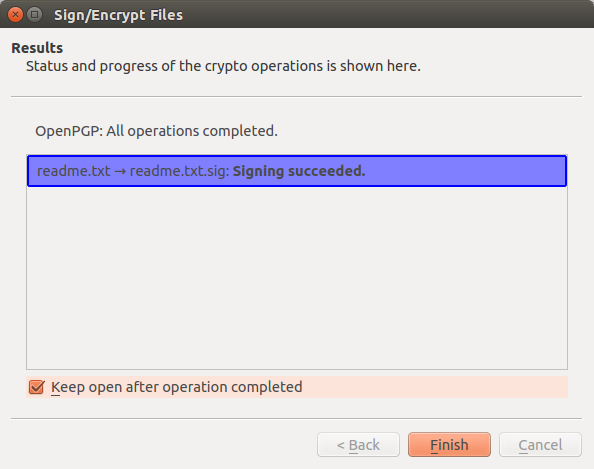
\includegraphics[width=0.8\linewidth]{Img/9}}
			\caption{Сообщение об успешном завершении.}
			\label{Img:9}
		\end{figure}
		
	\subsection{Импорт сертификата и его подпись}
	Для импорта сертификата выполним команду \textit{"File" "Import Certificates"} и выберем необходимый файл типа \textit{.asc} (рисунок \ref{Img:10}).
		
		\begin{figure}[h]
			\center{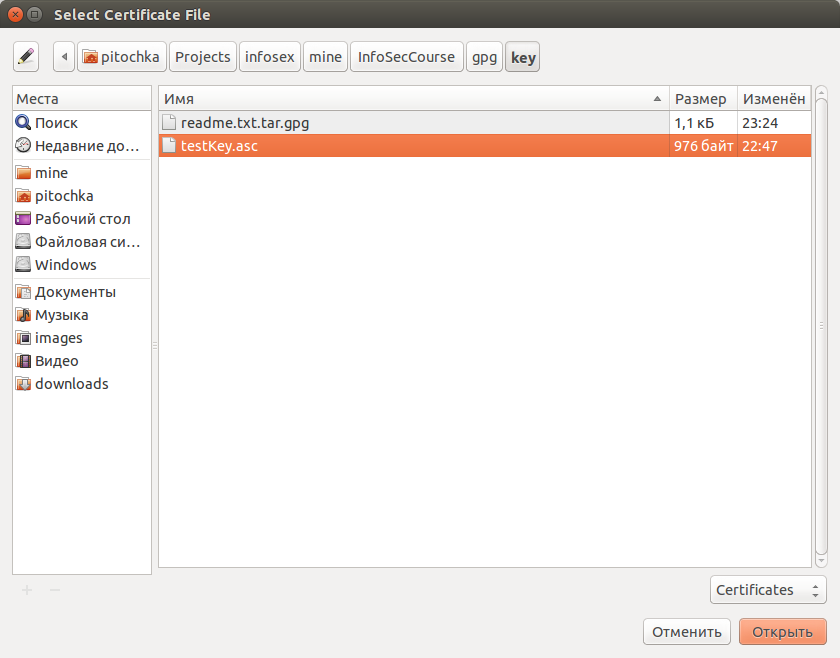
\includegraphics[width=0.8\linewidth]{Img/10}}
			\caption{Импорт сертификата.}
			\label{Img:10}
		\end{figure}	
	
	Подпишем этот сертификат как в предыдущем пункте. Теперь мы храним файл \textit{testKey.asc.sig}. Для проверки сертификата воспользуемся командой \textit{"File" -> "Decrypt/Verify Files"} и выберем подписанный ранее сертификат \textit{testKey.asc.sig} (рисунок \ref{Img:11}).
	
		\begin{figure}[h]
			\center{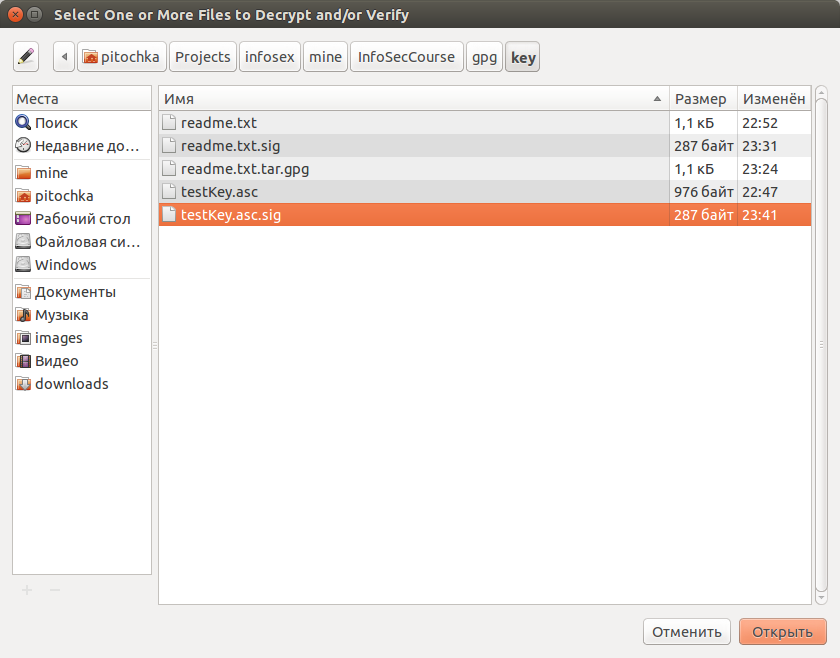
\includegraphics[width=0.8\linewidth]{Img/11}}
			\caption{Выбор сертификата для проверки.}
			\label{Img:11}
		\end{figure}	
		\pagebreak
		
	Проверка показывает, кем была осуществлена подпись (рисунок \ref{Img:12}).
		
		\begin{figure}[h]
			\center{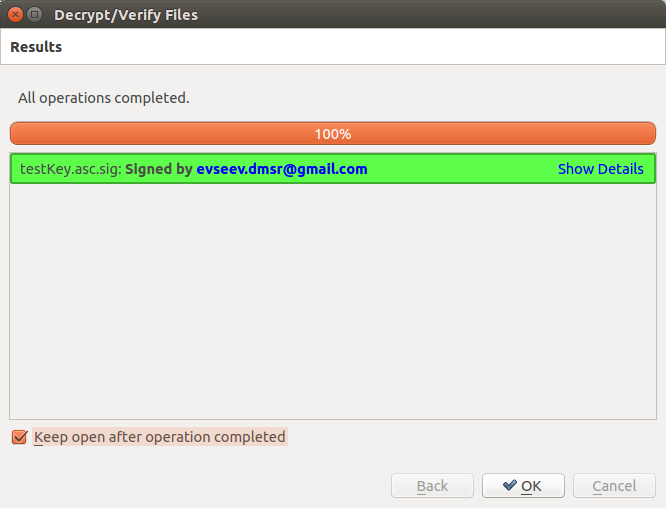
\includegraphics[width=0.8\linewidth]{Img/12}}
			\caption{Информация о подписи.}
			\label{Img:12}
		\end{figure}
	
	\subsection{Расшифровка файла}	
	Я с помощью моего ключа зашифровал документ и пытаюсь расшифровать \textit{readme.txt.gpg}. Командой \textit{"File" -> "Decrypt/Verify Files"} расшифруем документ. После расшифровки видем сообщение (рисунок \ref{Img:13}), также появился файл \textit{readme.txt}, который можно прочитать. 
	
		\begin{figure}[h]
			\center{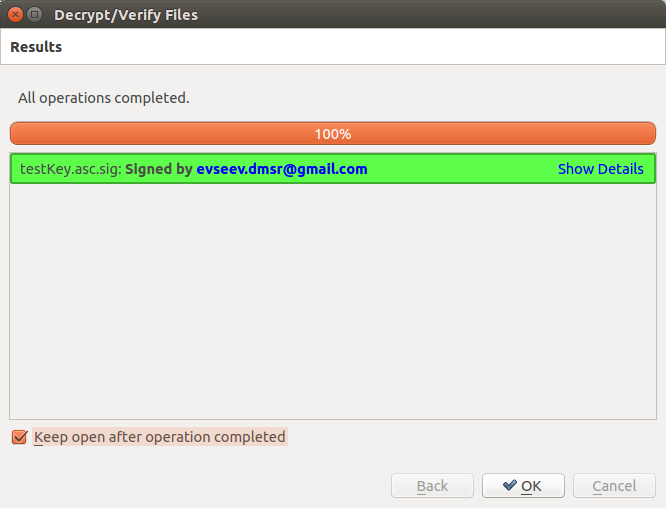
\includegraphics[width=0.8\linewidth]{Img/12}}
			\caption{Сообщение о расшифровке.}
			\label{Img:13}
		\end{figure}
	
	\section{Использование GNU Privacy handbook}
	Операции, проделанные с помощью графического интерфейса Kleopatra, можно повторить использую лишь консоль.
	
	Создание нового ключа производится с помощью команды (Рисунок \ref{Img:14}, \ref{Img:15}) \textit{gpg --gen-key}
	
	\begin{figure}[h]
		\begin{center}
			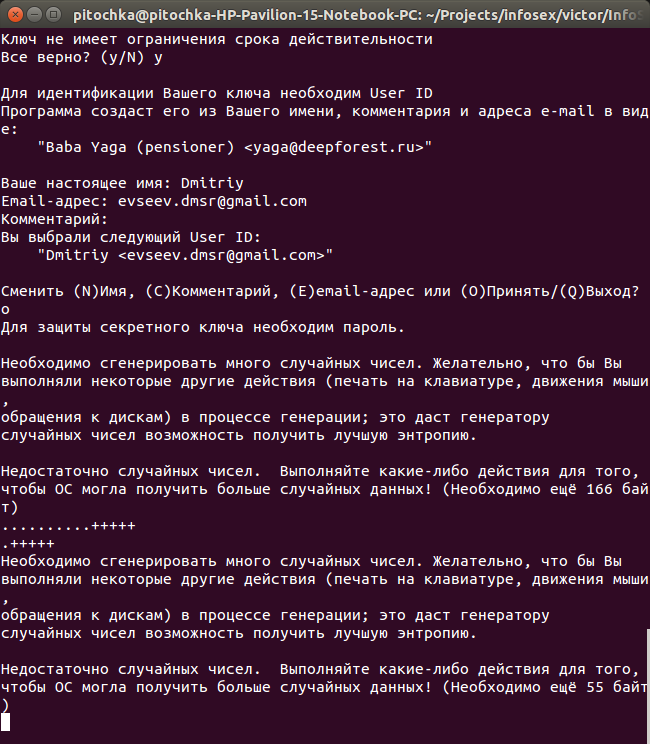
\includegraphics[width=0.8\textwidth]{Img/14}
			\caption{Создание ключа.}
			\label{Img:14}
		\end{center}
	\end{figure}
	
	\begin{figure}[h]
		\begin{center}
			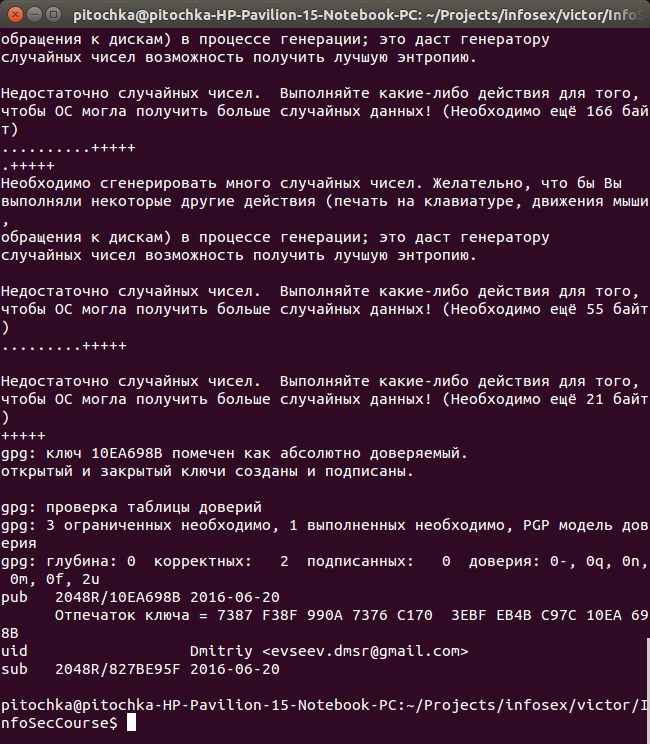
\includegraphics[width=0.8\textwidth]{Img/15} 
			\caption{Создание ключа.}
			\label{Img:15}
		\end{center}
	\end{figure}
	\pagebreak
	
	Для просмотра имеющихся в системе ключей необходимо воспользоваться командой (список ключей отображен на Рисунке \ref{Img:16}) \textit{gpg --list-keys}	
	
	\begin{figure}[h!]
		\begin{center}
			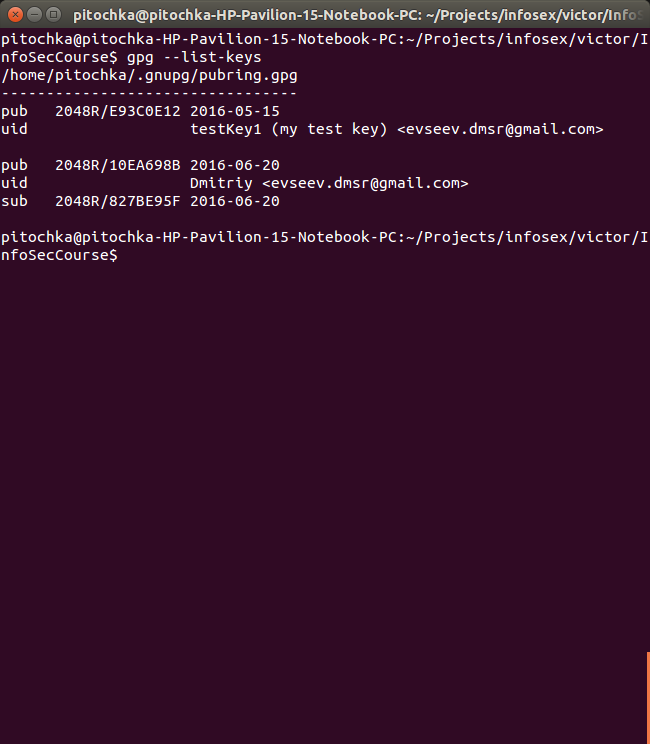
\includegraphics[width=0.5\textwidth]{Img/16}
			\caption{Список ключей.}
			\label{Img:16}
		\end{center}
	\end{figure}
	\pagebreak
	
	Экспорт ключей возможен с помощью команды \textit{gpg --export}	с различными опциями (например, вывод в файл, вид представления, выбор ключа для экспорта).
	
	Для импорта - \textit{gpg --import [filename]}
		 	
 	\section{Вывод}
 	В ходе лабораторной работы, используя пакет Gpg4win, я научилась создавать собственные ключевые пары и сертификаты на них; подписывать файлы и проверять подпись, а также зашифровывать и расшифровывать документы с помощью собственного сертификата или стороннего. Вышеперечисленные действия легко произвести как из графической обочки Kleopatra.
	
\end{document}